%%%%%%%%%%%%%%%%%%%%%%%%%
%% Header for standard beamer presentation
%%
%%  PresentationHeader.tex
%%
%%%%%%%%%%%%%%%%%%%%%%%%%

\documentclass[english,10pt]{beamer}

%%%%%%%%%%%%%%%%%%%%
%% Include general header where common packages are defined
%%%%%%%%%%%%%%%%%%%%

% general packages without options
\usepackage{amsmath,amssymb,bbm}




%%%%%%%%%%%%%%%%%%%%
%% Idem general commands
%%%%%%%%%%%%%%%%%%%%

%%% Commands

\newcommand{\noun}[1]{\textsc{#1}}


%% Math

% Operators
\DeclareMathOperator{\Cov}{Cov}
\DeclareMathOperator{\Var}{Var}
\DeclareMathOperator{\E}{\mathbb{E}}
\DeclareMathOperator{\Proba}{\mathbb{P}}

\newcommand{\Covb}[2]{\ensuremath{\Cov\!\left[#1,#2\right]}}
\newcommand{\Eb}[1]{\ensuremath{\E\!\left[#1\right]}}
\newcommand{\Pb}[1]{\ensuremath{\Proba\!\left[#1\right]}}
\newcommand{\Varb}[1]{\ensuremath{\Var\!\left[#1\right]}}

% norm
\newcommand{\norm}[1]{\| #1 \|}


% amsthm environments
\newtheorem{definition}{Definition}



%% graphics

% renew graphics command for relative path providment only ?
%\renewcommand{\includegraphics[]{}}






\usetheme{Warsaw}

\setbeamertemplate{footline}[text line]{}
\setbeamercolor{structure}{fg=purple!50!blue, bg=purple!50!blue}

\setbeamercovered{transparent}


% shortened command for a justified frame
\newcommand{\jframe}[2]{\frame{\frametitle{#1}\justify{#2}}}



%%%%%%%%%%%%%%%%%%%%%
%% Begin doc
%%%%%%%%%%%%%%%%%%%%%

\begin{document}



\title{Thesis Progress Meeting}


\author{J.~Raimbault$^{1,2}$}

\institute{$^{1}$G{\'e}ographie-cit{\'e}s (UMR 8504 CNRS)\\
$^{2}$LVMT (UMR-T 9403 IFSTTAR)}


\date{June 10th 2016}


%%%%%%%%%%%%%%%%%%%%%%%%%%%%%%%%
\begin{frame}
\titlepage
\end{frame}

%\begin{frame}
%\tableofcontents
%\end{frame}
%%%%%%%%%%%%%%%%%%%%%%%%%%%%%%%%



\section{Achieved Work}


%\item Gibrat-interaction Network Necessity [1.5w]\medskip
%\item Back on Memoire and ongoing projects [1w]\medskip
%\item Write proposal for China [0.5w]\medskip
%\item Cybergeo (conference May 26th) [1.5w]\medskip
%\item Finish side project (Transportation) [0.5w]


%NetworkNecessity	1,7
%Cybergeo	1,6
%Misc (AlgoSR, Scaling, Zipf, Gov, Tech, Chine, SFI prep)	0,5
%Spatial Stats	0,5
%Side (Transportation&Ecotox)	0,5
%Organisation/Workflow	0,3
%Seminar/Conference/Course	0,3
%General Bibliography	0,1



\jframe{Achieved Work (by projects)}{
\begin{itemize}
\item Cybergeo [1.6w] (ETA 1.5w)\medskip
\item Gibrat-interaction [1.7w] (ETA 1.5w)\medskip
\item Spatial Statistics [0.5w]\medskip
\item 
\end{itemize}
}



\section{Network Necessity}



\sframe{Network Necessity}{
\textbf{Simple toy models to test theoretical assumption of network necessity}

\medskip

$\rightarrow$ Extended Gibrat model for population growth within a city system (simplified Favaro-Pumain model or projected Cottineau-1.y.z model) with interactions. \textit{Idea :} Test if physical Network (feedback of physical flows) allows a better fit.

\medskip

\textbf{Rq. :} a lot of confusion on Gibrat Model :
\begin{enumerate}
\item Under classical independence assumptions, $Law(P)$ is known at any $t$ whatever the distribution of growth rates : no need to simulate).
\item Furthermore, various formulation are possible : independent realizations across cities of the same random process $P(t)$ with varying non-stationary parameters $\mu(t)$, with interdependence captured in recurrence relation between successive expectancies ; or multi-dimensional random process $(P_i(t))$ with covariance structure $\Covb{P_i}{P_j}$ estimated in time.
\end{enumerate}

}
%
%\sframe{Empirical Results}{
%\textit{Work on Pumain-INED French cities database.}
%\medskip
%\textbf{Growth Rates are more log-normal than normal ! } (simple likelihood tests) - in fact $\Delta \log P$ closer from levy fat-tail distribution.
%\medskip
%\textbf{Non-stationarity of correlations in time and space : }
%\smallskip
%\centering
%%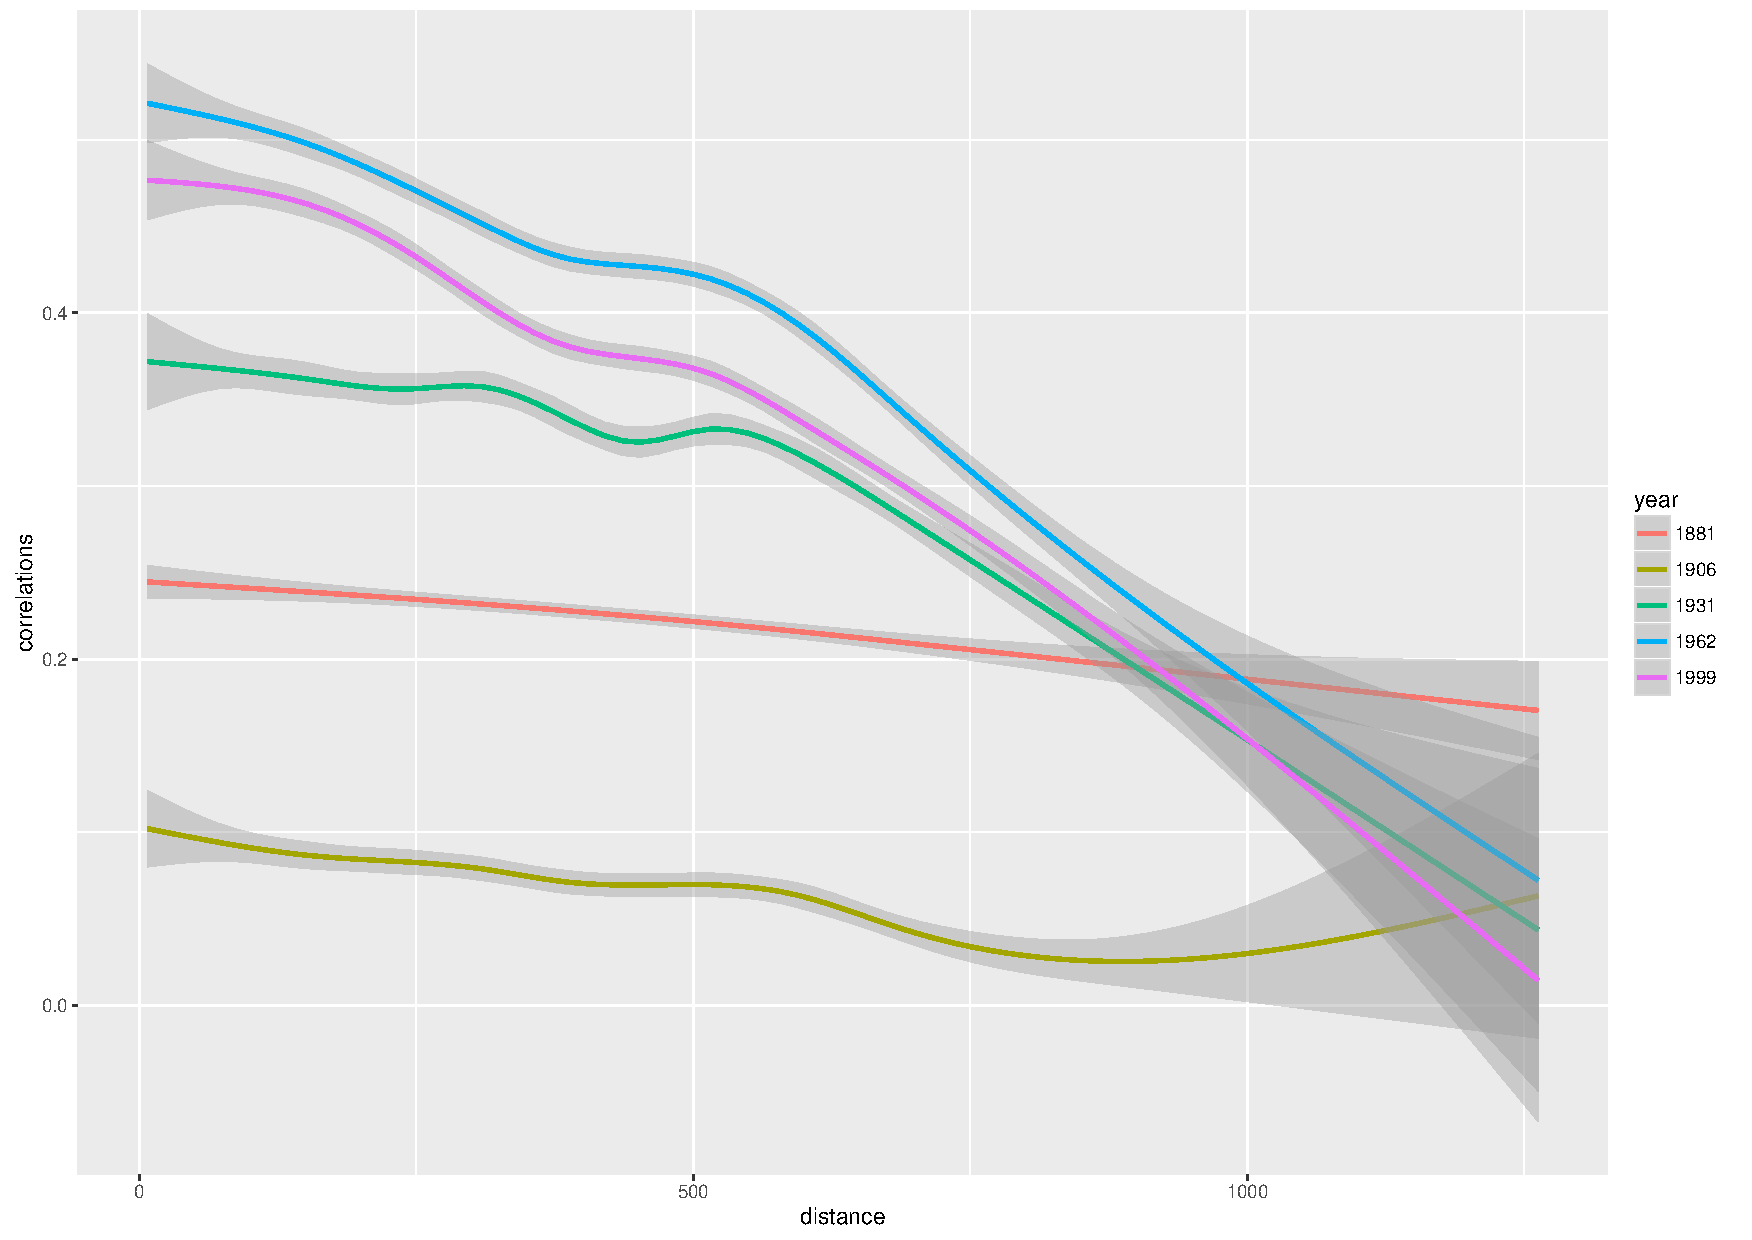
\includegraphics[width=0.6\textwidth]{figures/empirical_tsCorrelations}
%}

\sframe{First Modeling Results}{

Interaction model with $\Eb{\vec{P} (t+1)}= (r_0\cdot \mathbf{Id}+\mathbf{R})\Eb{\vec{P}(t)}$, specified with gravity interactions $\left(\mathbf{R}[\cdot]\right)_{ij} = \frac{1}{V_0}\cdot\left(\frac{\Eb{P_j}\Eb{P_i}}{P^2}\right)^{\gamma}\cdot \exp{\left(-\frac{d_ij}{d_0}\right)}$ (note : taking $\gamma=1$ yields linear formulation).

%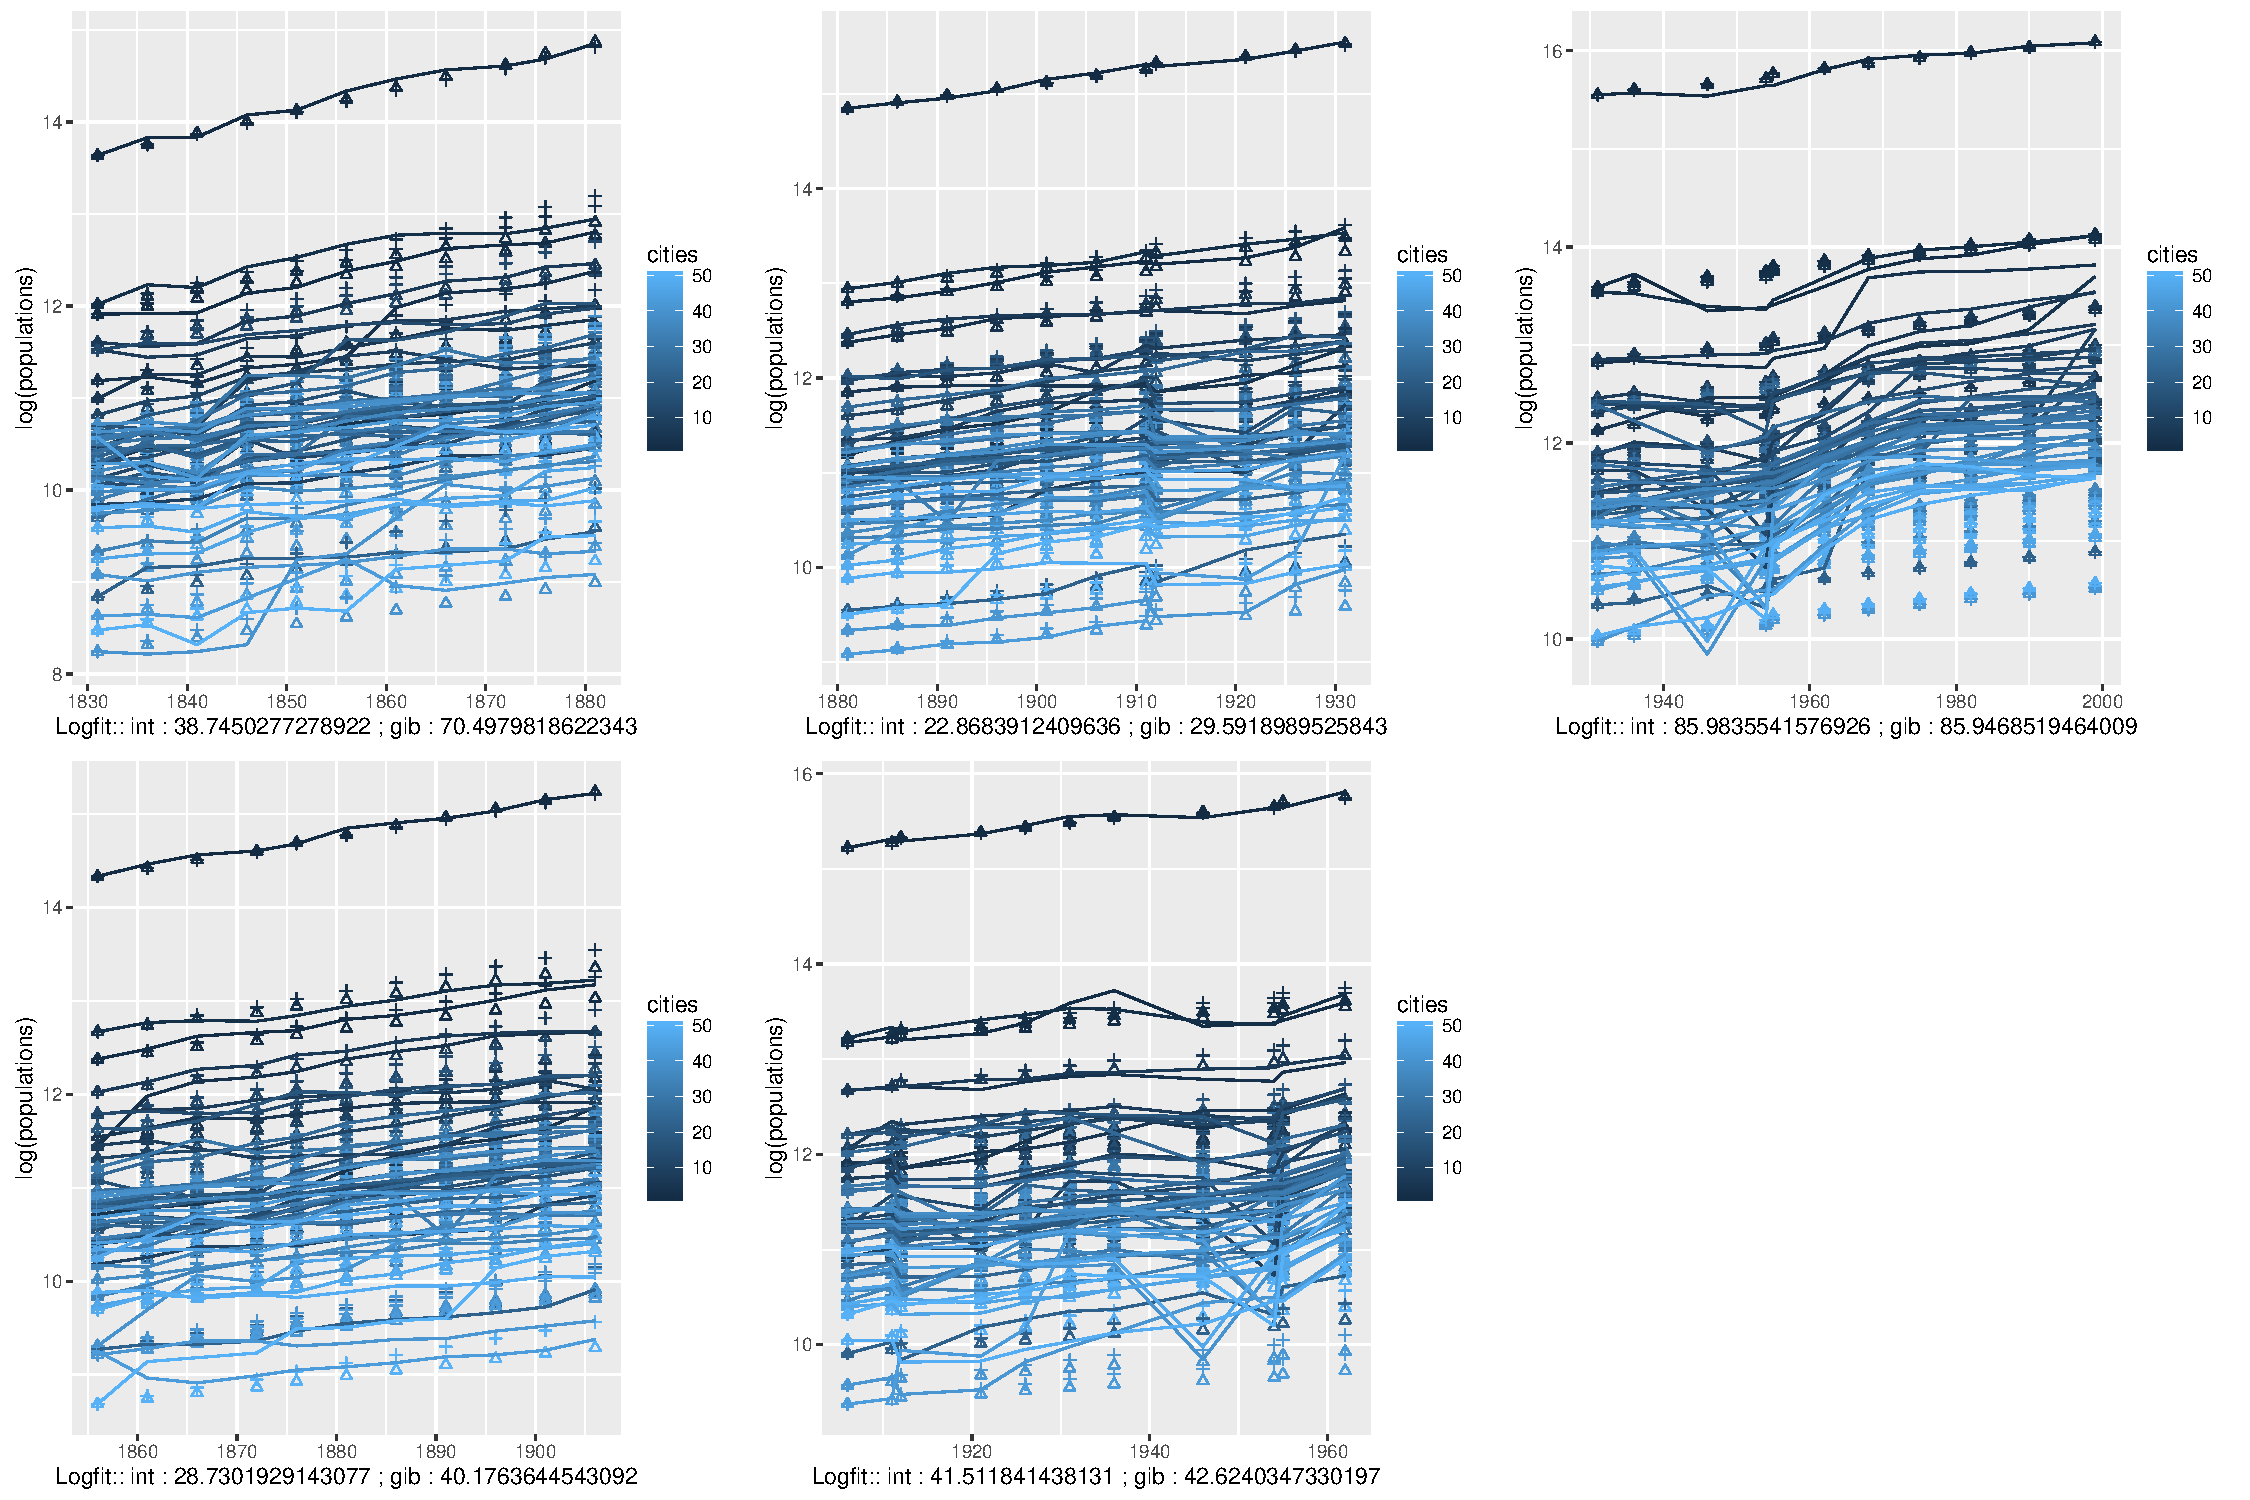
\includegraphics[width=0.8\textwidth]{figures/fit_intgib}
}

\sframe{Exploration}{
\textit{Gravity Only}

}

\sframe{Exploration}{
\textit{Feedback Only}

}

\sframe{Exploration}{
\textit{Feedback with fixed gravity : first evidences of network effects}

}


\sframe{Calibration}{
\textit{Gravity only}

% Pareto fronts

}

\sframe{Calibration}{
\textit{Feedback only}

% Pareto

}

\sframe{Calibration}{
\textit{Full Model, Iterative Calibration}

% fixed gravity Pareto Front

}

\sframe{Calibration}{
\textit{Full Model}

% full calib Pareto Front

}

\sframe{Profiles}{
\textit{Full Model}

% full calib Pareto Front

}


\sframe{Temporal moving window}{
\textit{Calibration by normalized periods (no war, same number of data points)}
%  gravity only calib

}

\sframe{Temporal moving window}{
% conditioned feedback by periods

% full calib period ? -> not sure.

}





%\sframe{Methodological Issue}{
%
%\textbf{Next step : } Introduce feedback terms due to effective physical flows passing through the city (in a first approximation only geographically computed with elevation data), test directly for network necessity. Fitting that model should also allow to quantify tunnel effect (strength of feedback).
%
%\bigskip
%
%\textbf{Methodological Flaw : } Issue with overfitting in models of simulations (seems to be an open question) : how do we know fit improvement is not only due to additional degree of freedom ? In stats : AIC provides Kullback-leibler information gain by correcting log-likelihood with number of parameters, nothing similar for models of simulation. Possible solutions :
%\small
%\begin{enumerate}
%\item Empirical version of AIC : Brutal version with empirical likelihood ? Estimation of statistical models on parameter space of each model of simulation, use of corresponding AIC ?
%\item Sparse non-linear machine learning to produce a kind of ``absolute'' benchmark explainable variance at a given number or parameters (rq : simple 2nd degree polynomial autoregressive model give far better results than two models above !)
%\end{enumerate}
%
%
%}
%


\section{Thesis Organisation}


\jframe{Thesis Organisation}{
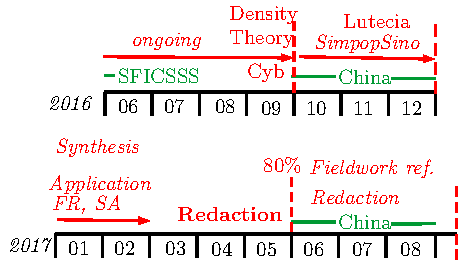
\includegraphics[width=\textwidth]{figures/edt}
}

%\jframe{Papers}{
%\begin{itemize}
%}



%%%%%%%%%%%%%%%%%%%%%%%%%%%%%%%%
\jframe{Next steps (until August 30th 2016)}{
\begin{itemize}
\item SFICSSS [4w] (+ holidays [2w])\medskip
\item Cybergeo Paper [1w]\medskip
\item Density Paper [1w]\medskip
\item Theoretical Paper [1w]\medskip
\item Static Correlations (presentation at RGS conference on 31th) [1w]\medskip
\item China project [1w]\medskip
\end{itemize}
}






%%%%%%%%%%%%%%%%%%%%%%%%%%%%%%%%
%\begin{frame}[allowframebreaks]
%\frametitle{References}
%\bibliographystyle{apalike}
%\bibliography{/Users/Juste/Documents/ComplexSystems/CityNetwork/Biblio/Bibtex/CityNetwork}
%\end{frame}
%%%%%%%%%%%%%%%%%%%%%%%%%%%%%%%%


\end{document}




